\documentclass[10pt,a4paper]{article}
\usepackage[utf8]{inputenc}
\usepackage{amsmath}
\usepackage{amsfonts}
\usepackage{amssymb}
\usepackage{amsthm}
\usepackage{float}
\usepackage{mathtools}
\usepackage{geometry}[margin=1in]
\usepackage{xspace}
\usepackage{tikz}
\usepackage{mathrsfs}
\usetikzlibrary{shapes, arrows, decorations.pathmorphing}
\usepackage[parfill]{parskip}
\usepackage{subcaption}
\usepackage{stmaryrd}
\usepackage{marvosym}
\usepackage{dsfont}

\newcommand{\st}{\text{ s.t. }}
\newcommand{\contr}{\lightning}
\newcommand{\im}{\mathfrak{i}}
\newcommand{\R}{\mathbb{R}}
\newcommand{\Q}{\mathbb{Q}}
\newcommand{\C}{\mathbb{C}}
\newcommand{\F}{\mathbb{F}}
\newcommand{\K}{\mathbb{K}}
\newcommand{\N}{\mathbb{N}}
\newcommand{\Z}{\mathbb{Z}}
\renewcommand{\H}{\mathds{H}}
\newcommand{\nequiv}{\not\equiv}
\newcommand{\powset}{\mathcal{P}}
\renewcommand{\th}[1][th]{\textsuperscript{#1}\xspace}
\newcommand{\from}{\leftarrow}
\newcommand{\legendre}[2]{\left(\frac{#1}{#2}\right)}
\newcommand{\ow}{\text{otherwise}}
\newcommand{\imp}[2]{\underline{\textit{#1.}$\implies$\textit{#2.}}}
\let\oldexists\exists
\renewcommand{\exists}{\oldexists\;}
\renewcommand{\hat}{\widehat}
\renewcommand{\tilde}{\widetilde}
\newcommand{\one}{\mathds{1}}
\newcommand{\under}{\backslash}
\newcommand{\injection}{\hookrightarrow}
\newcommand{\surjection}{\twoheadrightarrow}
\newcommand{\jacobi}{\legendre}
\newcommand{\floor}[1]{\lfloor #1 \rfloor}
\newcommand{\ceil}[1]{\lceil #1 \rceil}
\newcommand{\cbrt}[1]{\sqrt[3]{#1}}

\DeclareMathOperator{\ex}{ex}
\DeclareMathOperator{\id}{id}
\DeclareMathOperator{\upper}{Upper}
\DeclareMathOperator{\dom}{dom}

\DeclareMathOperator{\charr}{char}
\DeclareMathOperator{\Image}{im}
\DeclareMathOperator{\ord}{ord}
\DeclareMathOperator{\lcm}{lcm}
\let\emph\relax
\DeclareTextFontCommand{\emph}{\bfseries\em}

\newtheorem{theorem}{Theorem}[section]
\newtheorem{lemma}[theorem]{Lemma}
\newtheorem{corollary}[theorem]{Corollary}
\newtheorem{proposition}[theorem]{Proposition}
\newtheorem{conjecture}[theorem]{Conjecture}

\tikzset{sketch/.style={decorate,
 decoration={random steps, amplitude=1pt, segment length=5pt}, 
 line join=round, draw=black!80, very thick, fill=#1
}}

\title{Graph Theory}
\begin{document}
\maketitle
\section{Introduction}
\subsection*{Definitions}
Formally, we define a \emph{graph} to be an ordered pair $G = (V, E)$ where $E \subseteq V^{(2)} \coloneqq \{ Y \subseteq V : |Y| = 2\}$\\\\
e.g. $V = \{a,b,c,d\}, E = \left\{\{a,b\},\{a,c\},\{a,d\},\{b,c\}\right\}$\\
\begin{center}
\tikz{
\node (a) at (0,1) [circle, draw] {a};
\node (b) at (1,1) [circle, draw] {b};
\node (c) at (0,0) [circle, draw] {c};
\node (d) at (1,0) [circle, draw] {d};
\draw (a) edge (b) (a) edge (c) (a) edge (d) (b) edge (c);
}
\end{center}
The set \emph{$V(G)$} is the \emph{vertex set} of $G$ and \emph{$E(G)$} is the \emph{edge set}.\\
The \emph{order} of $G$ is $|V(G)|$, often written $|G|$.\\
The \emph{size} of G is $|E(G)|$, often written $e(G)$.\\
Note that for the purposes of this course, all graphs will be finite.

This definition that we use precludes:
\begin{itemize}
\item Having more than one edge between the same two vertices
\item Having an edge with both ends at the same vertex
\end{itemize}
\begin{figure}[h]
\begin{center}
\tikz{
\node (a) at (0,1) [circle,draw] {};
\node (b) at (1,1) [circle,draw] {};
\node (c) at (0.5,0.2) [circle,draw] {};
\node (d) at (1.5,0.5) [circle,draw] {};
\draw (a) edge[bend left] (b);
\draw (a) edge[bend right, red] (b);
\draw (a) edge (c);
\draw (b) edge (c);
\draw (c) edge (d);
\draw[red] (d.-60) arc (210:180+330:3mm);
}
\end{center}
\caption*{These 2 red edges are not allowed}
\end{figure}

Some authors allow graphs to have these features, and call what we're studying \emph{simple graphs}.

It's easier to write the edge $\{a,b\}$ as $ab$.\\
If $ab \in E(G)$, we say that ``$a$ is \emph{adjacent} to $b$'', and vice versa. We might write $ab \in G$.

Edges containing a vertex $x$ are said to be \emph{incident} to $x$ and to each other.

Two graphs $G, H$ are said to be \emph{isomorphic} if there exists a bijection\\ $f:V(G) \rightarrow V(H) \st uv\in E(G) \iff f(u)f(v) \in E(H)$.

There are some canonical graphs:

\begin{tabular}{c|c|c|c}
Name & Notation & Order & Size \\\hline
Empty graph & $E_n$ & $n$ & 0 \\
Complete graph & $K_n$ & $n$ & $\binom{n}{2}$ \\
Path & $P_n$ & $n$ & $n-1$ \\
Circuit & $C_n$ & $n$ & $n$
\end{tabular}\\
\begin{figure}
\begin{subfigure}{.3\textwidth}
\centering
\scalebox{1.5}{
\tikz{
\node (a) at (0,0.6) [circle, draw] {};
\node (b) at (0.6,1) [circle, draw] {};
\node (c) at (1.2,0.6) [circle, draw] {};
\node (d) at (0.9,0) [circle, draw] {};
\node (e) at (0.3,0) [circle, draw] {};
\draw (a) edge (b) edge (c) edge (d) edge (e);
\draw (b) edge (c) edge (d) edge (e);
\draw (c) edge (d) edge (e);
\draw (d) edge (e);
}}
\caption{$K_5$}
\end{subfigure}
\begin{subfigure}{.3\textwidth}
\centering
\scalebox{1.5}{
\tikz{
\node (a) at (0,0.5) [circle, draw] {};
\node (b) at (1,0) [circle, draw] {};
\node (c) at (2,0.5) [circle, draw] {};
\node (d) at (3,0) [circle, draw] {};
\draw (a) edge (b) (b) edge (c) (c) edge (d);
}}
\caption{$P_4$}
\end{subfigure}
\begin{subfigure}{.3\textwidth}
\centering
\scalebox{1.5}{
\tikz{
\node (a) at (0.2,0.5) [circle, draw] {};
\node (b) at (0.5,1) [circle, draw] {};
\node (c) at (1,1) [circle, draw] {};
\node (d) at (1.3,0.5) [circle, draw] {};
\node (e) at (1,0) [circle, draw] {};
\node (f) at (0.5,0) [circle, draw] {};
\draw (a) edge (b) (b) edge (c) (c) edge (d) (d) edge (e) (e) edge (f) (f) edge (a);
}}
\caption{$C_6$}
\end{subfigure}
\end{figure}

A \emph{subgraph} of $G$ is another graph $H$ with $V(H) \subseteq V(G), E(H) \subseteq E(G)$. (Ever graph of order $\leq n$ is a subgraph of $K_n$).\\
The subgraph of G \emph{induced by} $W \subseteq V(G)$, written $G[W]$ is the graph $(W, E(G)\cap W^{(2)})$, i.e. the vertex set $W$ and all edges of $G$ lying inside $W$.

A graph is \emph{connected} if there is a $u-v$ path (a path from $u$ to $v$ in $G$ for every pair $u,v \in V(G)$.\\
The \emph{components} of $G$ are the maximal connected subgraphs of $G$ (induced by the equivalence classes of the relation $u\leftrightarrow v \iff u = v$ or there is a $u-v$ path).

E.g.:\\
\tikz{
\node (a) at (0,0) [circle, draw] {};
\node (b) at (0.5,1) [circle, draw] {};
\node (c) at (1,0) [circle, draw] {};
\node (d) at (1.5,1) [circle, draw] {};
\node (e) at (2.5,1) [circle, draw] {};
\node (f) at (2,0) [circle, draw] {};
\node (g) at (3,1) [circle, draw] {};
\node (h) at (4,0) [circle, draw] {};
\node (i) at (5,0.5) [circle, draw] {};
\draw (a) edge (b) edge (c) (b) edge (c);
\draw (d) edge (e) (e) edge (f);
\draw (g) edge (h);
}\\
has 4 components.

A \emph{forest} is a graph containing no circuit.\\
A \emph{tree} is a connected forest, i.e. the components of a forest are trees.\\
Equivalently, a tree is a connected circuit-free graph. This bring us on to our first theorem of the course:

\begin{theorem}
The following are equivalent:
\begin{enumerate}
\item $G$ is a tree
\item $G$ is a minimal connected (connected, but the removal of any edge kills connectivity)
\item $G$ is maximal circuit-free (the addition of any edge creates a circuit)
\end{enumerate}
\end{theorem}

\begin{proof}
\subsubsection*{$(a) \implies (b)$}
Let $G$ be connected and circuit free. Suppose $uv\in G$ and $G-uv$ is connected. Then there is a $u-v$ path $P$ in $G-uv$, so $G$ contains the circuit $P+uv$ \contr ($G$ circuit free)\\
\therefore $G$ is minimal connected.
\subsubsection*{$(b) \implies (a)$}
Let $G$ be minimal connected, but suppose $G$ has a circuit $C$, with $xy \in C$. Let $u, v \in V(G)$. There is a $u-v$ path $P$ in $G$.\\
If $xy \notin P$, then $P$ joins $u$ to $v$ in $G-xy$.\\
If $xy \in P$, then $(P\cup C)-xy$ contains a $u-v$ path in $G-xy$.\\
Hence $G-xy$ is connected \contr ($G$ \emph{minimal} connected).\\
\therefore $G$ is circuit free, and connected by hypothesis, hence a tree.
\subsubsection*{$(a) \implies (c)$}
Let $G$ be a tree. If $uv \notin E(G)$ there is a path $P$ in $G$ from $u$ to $v$, so $P+uv$ is circuit in $G+uv$, so $G$ is maximal circuit free.
\subsubsection*{$(c) \implies (a)$}
Let $G$ be maximal circuit free. Let $u,v \in V(G)$. Either $uv \in E(G)$ or $G+uv$ has a circuit $C$, so $C-uv$ is a $u-v$ path in $G$, and so $G$ is connected, and hence a tree.
\end{proof}

A subgraph $T$ of a graph $G$ is said to be \emph{spanning} if $V(T) = V(G)$, i.e. the subgraph touches every vertex of $G$
\begin{corollary}
A graph is connected if and only if it has a spanning tree.
\end{corollary}
\begin{proof}
\item
\begin{itemize}
\item{$\implies$} $T$ is connected as it is a tree, and is spanning, so all vertices in $G$ are connected via $T$.
\item{$\Longleftarrow$} Remove edges from $G$ to obtain a minimal connected spanning subgraph $T$. By \textbf{1.1} $T$ is a tree.
\end{itemize}
\end{proof}

The set of \emph{neighbours} of a vertex $v$ is $\Gamma(v) = \{w: vw\in E(G)\}$.\\
The \emph{degree} $d(v)$ is the number of neighbours of $v$, $|\Gamma(v)|$\\
The minimum and maximum degrees in $G$ are denoted by $\delta(G)$ and $\Delta(G)$. \\
If $\delta(G) = \Delta(G) = k$, i.e. $d(v)=k \forall v$ we say $G$ is \emph{$k$-regular}. A \emph{regular} graph is one that is $k$-regular for some $k$. If a graph is $3$-regular, it is called \emph{cubic}.\\
The degrees of the graph written in some order form a \emph{degree sequence} of $G$.

\begin{lemma}[lemma Lemma]
\begin{align*}
\sum_{v\in G} d(v) = 2e(G)
\end{align*}
\end{lemma}
\begin{proof}
Each edge has $2$ vertices at the end, so contributes $2$ to the sum of all degrees.
\end{proof}
A \emph{leaf} is a vertex of degree $1$.
\begin{theorem}
Every tree $T$ with $|T|\geq 2$ has at least two leaves.
\end{theorem}
\begin{proof}
We note $T$ is connected so $\delta(T) \geq 1$. Let $x_1$ be a vertex (a leaf if there is one). Let $x_1x_2\ldots x_k$ be a maximal path from $x_1$. $T$ is circuit-free so none of $x_1,\ldots,x_{k-2}$ is in $\Gamma(x_k)$, and $x_k$ has no other neighbours except for $x_{k-1}$, otherwise this path can be extended, hence $\Gamma(x_k) = \{x_{k-1}\}$, so $x_k$ is a leaf. Repeat the proof starting at $x_k$ for a second leaf.
\end{proof}

\begin{corollary}
A tree of order $n$ has size $n-1$
\end{corollary}
\begin{proof}
\item
This is true for $n = 1, 2$ by inspection, as there is only 1 tree:

\begin{figure}[h]
\begin{subfigure}{.5\textwidth}
\centering
\tikz{
\node (a) at (0,0) [circle, draw] {};
}
\caption{$n=1$}
\end{subfigure}
\begin{subfigure}{.5\textwidth}
\centering
\tikz{
\node (a) at (0,0) [circle, draw] {};
\node (b) at (1,0) [circle, draw] {};
\draw (a) edge (b);
}
\caption{$n=2$}
\end{subfigure}
\end{figure}
Let $|T| \geq 3$. By \textbf{1.3} $T$ has a leaf $v$. Then $T-v$ is certainly circuit free and connected, because the $x-y$ path in $T$ uses $v$ if and only if $x$ or $y$ is $v$. Hence the corollary follows by induction.
\end{proof}

\begin{corollary}
The following are equivalent for a graph $G$ of order $n$:
\begin{enumerate}
\item $G$ is a tree
\item $G$ is connected and $e(G) = n-1$
\item $G$ is acyclic and $e(G) = n-1$
\end{enumerate}
\end{corollary}
\begin{proof}\item
\begin{itemize}
\item{$(1) \implies (2),(3)$:} True by definition and \textbf{1.5}.
\item{$(2) \implies (1)$:} By \textbf{1.2} $G$ contains a spanning tree $T$. By \textbf{1.5} $e(T) = e(G)$ so $T=G$
\item{$(3) \implies (1)$:} Add edges to $G$ to get a graph $G'$ maximal acyclic. By \textbf{1.1} $G'$ is a tree, so by \textbf{1.5} $e(G') = n-1 = e(G)$, so $G' = G$.
\end{itemize}
\end{proof}

\subsection*{How many graphs of order $n$ are there?}
Let the vertex set be $[n] \coloneqq \{1,2,\ldots,n\}$. E.g. for $n=3$  we have:\\
\begin{figure}[h]
\begin{subfigure}{0.12\textwidth}
\centering
\tikz{
\node (1) at (0,0) [circle, draw] {$1$};
\node (2) at (1,0) [circle, draw] {$2$};
\node (3) at (0.5,0.667) [circle, draw] {$3$};
}
\end{subfigure}
\begin{subfigure}{0.12\textwidth}
\centering
\tikz{
\node (1) at (0,0) [circle, draw, blue] {$1$};
\node (2) at (1,0) [circle, draw, blue] {$2$};
\node (3) at (0.5,0.667) [circle, draw, blue] {$3$};
\draw[blue] (1) edge (2);
}
\end{subfigure}
\begin{subfigure}{0.12\textwidth}
\centering
\tikz{
\node (1) at (0,0) [circle, draw, blue] {$1$};
\node (2) at (1,0) [circle, draw, blue] {$2$};
\node (3) at (0.5,0.667) [circle, draw, blue] {$3$};
\draw[blue] (1) edge (3);
}
\end{subfigure}
\begin{subfigure}{0.12\textwidth}
\centering
\tikz{
\node (1) at (0,0) [circle, draw, blue] {$1$};
\node (2) at (1,0) [circle, draw, blue] {$2$};
\node (3) at (0.5,0.667) [circle, draw, blue] {$3$};
\draw[blue] (2) edge (3);
}
\end{subfigure}
\begin{subfigure}{0.12\textwidth}
\centering
\tikz{
\node (1) at (0,0) [circle, draw, red] {$1$};
\node (2) at (1,0) [circle, draw, red] {$2$};
\node (3) at (0.5,0.667) [circle, draw, red] {$3$};
\draw[red] (2) edge (3);
\draw[red] (1) edge (2);
}
\end{subfigure}
\begin{subfigure}{0.12\textwidth}
\centering
\tikz{
\node (1) at (0,0) [circle, draw, red] {$1$};
\node (2) at (1,0) [circle, draw, red] {$2$};
\node (3) at (0.5,0.667) [circle, draw, red] {$3$};
\draw[red] (2) edge (3);
\draw[red] (1) edge (3);
}
\end{subfigure}
\begin{subfigure}{0.12\textwidth}
\centering
\tikz{
\node (1) at (0,0) [circle, draw, red] {$1$};
\node (2) at (1,0) [circle, draw, red] {$2$};
\node (3) at (0.5,0.667) [circle, draw, red] {$3$};
\draw[red] (1) edge (3);
\draw[red] (1) edge (2);
}
\end{subfigure}
\begin{subfigure}{0.12\textwidth}
\centering
\tikz{
\node (1) at (0,0) [circle, draw, green!70!black] {$1$};
\node (2) at (1,0) [circle, draw, green!70!black] {$2$};
\node (3) at (0.5,0.667) [circle, draw, green!70!black] {$3$};
\draw[green!70!black] (2) edge (3);
\draw[green!70!black] (1) edge (2);
\draw[green!70!black] (1) edge (3);
}
\end{subfigure}
\end{figure}\\
There are $2^{\binom{n}{2}}$ \emph{labelled} graphs of order $n$ - $\binom{n}{2}$ potentially edges, each of which we can independently choose to include or not.\\
However, there are only $4$ unlabelled graphs of order $3$ - all the graphs of the same colour are essentially the same, just with different labels given to the vertices. In general we must count the number of orbits amongst labelled graphs under the action of a group, using Burnside's Lemma. In fact, it turns out this number is asymptotic to $2^{\binom{n}{2}}/n!$

\subsection*{How many trees of order $n$ are there?}
\begin{theorem}[Cayley]
There are $n^{n-2}$ labelled tress of order $n$.
\end{theorem}
\begin{proof}(Pr\"ufer, Non-examinable)\\
We construct a bijection between trees strings length $n-2$ over the alphabet $n$.
\begin{itemize}
\item{\underline{Tree $\rightarrow$ string:}} Select the lowest leaf, write down its neighbour, remove that leaf, and repeat until only one edge is left.
\begin{center}
\tikz{
\node (1) at (5,2) [circle, draw] {$1$};
\node (2) at (6.5,2.3) [circle, draw] {$2$};
\node (3) at (5.1,1) [circle, draw] {$3$};
\node (4) at (6,0) [circle, draw] {$4$};
\node (5) at (3,1) [circle, draw] {$5$};
\node (6) at (8,2) [circle, draw] {$6$};
\node (7) at (1,2) [circle, draw] {$7$};
\node (8) at (6.1,1.5) [circle, draw] {$8$};
\node (9)  at (8,1) [circle, draw] {$9$};
\node (10) at (1,0.5) [circle, draw] {$10$};
\node (11) at (4,0.3) [circle, draw] {$11$};
\draw (1) edge (3);
\draw (2) edge (8);
\draw (3) edge (5) edge (8) edge (11);
\draw (4) edge (11);
\draw (5) edge (10) edge (7);
\draw (6) edge (8);
\draw (8) edge (9);
}
\end{center}
Here, we would get the string $3, 8, 11, 8, 5, 8, 3, 5, 10$. Each vertex is written down $d(n)-1$ times
\item{\underline{String $\rightarrow$ tree:}} Mark all vertices "unused". Then repeatedly choose the smallest unused vertex not in the string. Join it to the first vertex in the string. Mark it as used. Delete first vertex in the string.
\end{itemize}
\end{proof}

A graph is \emph{$r$-partite} if its vertices can be partitioned into $r$ classes so that no edge lies within a class. In the special case where $r=2$ we call the graph \emph{bipartite}. Remarkably, we can characterise all bipartite graphs.
\begin{theorem}
A graph is bipartite if and only if it contains no odd circuit.
\end{theorem}
\begin{proof}
For the ``only if" part, in a bipartite graph the vertices of a circuit alternate between the two classes, otherwise an edge would lie in a class. Hence any circuit must be of even length.

For the ``if" part, take some graph $G$, pick a vertex $v_0$ and let $V_i = \{v : d(v_0,v) = i\}$ where $d(v_0,v)$ is the \emph{distance} of $v$ from $v_0$, i.e. the length of a shortest $v_0-v$ path. 
\begin{center}
\tikz{
\node[circle, draw] (v0) at (0,0) {$v_0$};
\node[black!75!white, ellipse, draw, minimum width=0.3cm, minimum height=2cm] (v1) at (2,0) {$V_1$};
\node[black!50!white, ellipse, draw, minimum width=0.3cm, minimum height=2cm] (v2) at (4,0) {$V_2$};
\node[black!25!white, ellipse, draw, minimum width=0.3cm, minimum height=2cm] (v3) at (6,0) {$V_3$};
\node[ellipse, minimum width=0.3cm+15pt, minimum height=2cm] (v4) at (8,0) {};
\node (l) at (8,0) {$\cdots$};
\draw[black!88!white] (v0) edge (v1.110) edge (v1) edge (v1.250);
\draw[black!63!white] (v1.70) edge (v2.110) (v1.290) edge (v2.250) (v1) edge (v2);
\draw[black!38!white] (v2.70) edge (v3.110) (v2.290) edge (v3.250) (v2) edge (v3);
\draw[black!13!white] (v3.70) edge (v4.110) (v3.290) edge (v4.250) (v3) edge (v4);
}
\end{center}
If $G$ is connected, $V_0, V_1, V_2, \ldots$ partition $V(G)$. (Note $V_0 = \{v_0\}$). There is no edge between $V_i$ and $V_{i+k}$ if $k \geq 2$ by construction. Suppose $G$ has no odd circuit. Then $G$ cannot have an edge inside one of the $V_i$: if $u,v \in V_i$ and $uv\in G$, then there is a way of getting from $v_0$ to itself in an odd number of steps. $v_0 \xrightarrow{i} u \xrightarrow{1} v \xrightarrow{i} v_0$. This must contain an odd circuit: let the first path be $v_0=a_0,a_1,a_2,\ldots, a_{i-1}, u$ and the second be $v_0=b_0,b_1,b_2,\ldots,b_{i-1},v$, and let $k = \max\{j: a_j=b_j\}$, so $0\leq k <i$. Then $a_k, a_{k+1},\ldots,u,v,b_{i-1},\ldots,b_k=a_k$ is an odd cycle.  Hence we can let our two classes be $\cup_i V_{2i}$ and $\cup_i V_{2i+1}$, and $G$ is bipartite.
\end{proof}

An \emph{Euler cycle} as a ``walk" around all the edges of a graph returning to the starting point so that every vertex is visited and every edge is used precisely once.
\begin{figure}
\centering
\scalebox{0.8}{
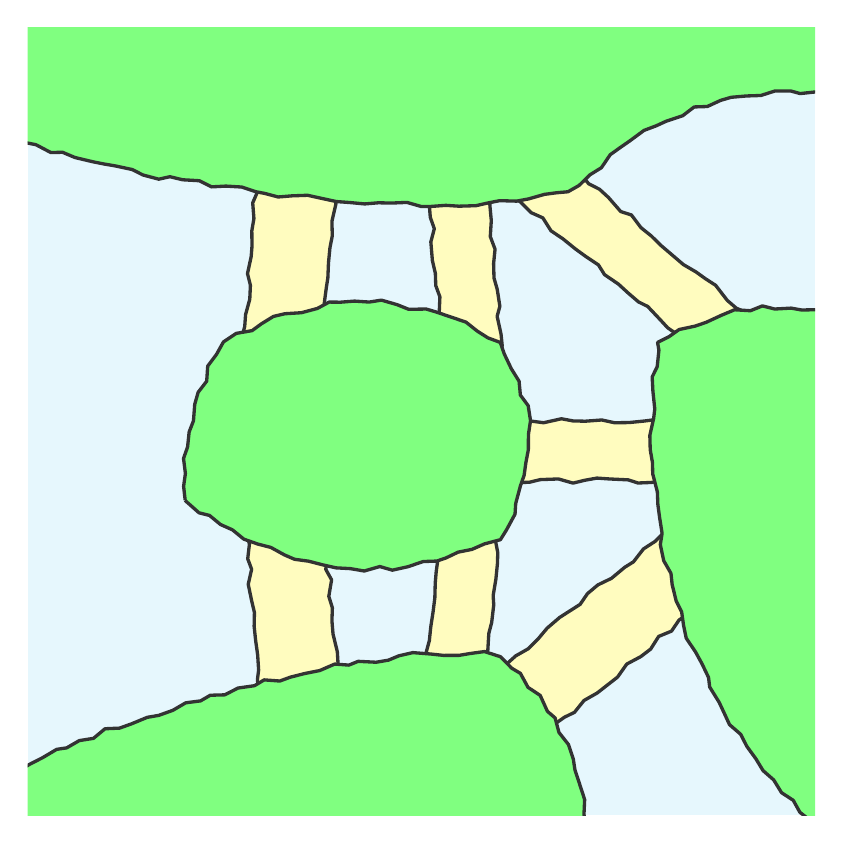
\begin{tikzpicture}

\clip [preaction={fill=cyan!10}] (0,0) rectangle (10,10);

\foreach \p/\r/\w/\h in 
  {(3,1)/5/1/4, (3,9)/-5/1/-4, (5,1)/-5/0.75/4, (5,9)/5/0.75/-4, 
  (5,5)/-90/0.75/4, (5,1)/-50/1/4, (6,8)/50/0.75/-4}
\draw [sketch=yellow!25]
   [shift={\p}, rotate=\r] rectangle +(\w,\h);

\draw [sketch=green!50]
  (-1,-1) -- (-1,0) to [bend left, looseness=0.5] (6,2) to [bend left] (7,-1) 
  (11,-1) to [bend left] (8,6) to [bend left] (11,6) -- cycle
  (-1,9) to [bend right, looseness=0.5] (7,8) to [bend left] 
  (11,9) -- (11,11) -- (-1,11) -- cycle
  (2,4) to [bend left, looseness=0.5] (2.5,6) to [bend left] 
  (6,6) to [bend left] (6,3.5) to [bend left] (2,4) -- cycle;
\end{tikzpicture}
}
\caption*{The bridges of K\"onigsberg, which inspired this problem}
\end{figure}

A graph is \emph{Eulerian} if it is a single vertex or has an Euler cycle.
\begin{theorem}
A graph is Eulerian if and only if it is connected and every vertex has even degree
\end{theorem}
\begin{proof}
The forwards direction is clear: an Eulerian graph must be connected, and for every time we enter a vertex along an edge we must also leave that vertex, so each vertex has even degree.

We do the opposite direction by induction on $e(G)$. Since $\delta(G) \geq 2$ by \textbf{1.4} $G$ is not a tree and so has a circuit $C$. Every vertex of $G-E(C)$ has even degree, so by induction each component of $G-E(C)$ is Eulerian. Now set off walking round $C$, taking the time to traverse any Euler cycle of $G-E(C)$ when first encountered. Since $G$ is connected, this gives an Euler cycle of $G$.
\end{proof}

A graph that can be drawn in the plane without edges crossing is \emph{planar}. A graph drawn in the plane is a \emph{plane graph}. A \emph{face} of a plane graph is a connected region of $\R^2\setminus G$. We define the \emph{size} of a face to be the number of edges it has.\\
E.g.:
\begin{figure}[h]
\begin{subfigure}{.5\textwidth}
\centering
\tikz{
\node (a) at (0,2) [circle, draw] {};
\node (b) at (1.5,0) [circle, draw] {};
\node (c) at (3,2) [circle, draw] {};
\node (d) at (4.5,0) [circle, draw] {};
\node (e) at (6,2) [circle, draw] {};
\draw (a) edge (b) edge (c) (b) edge (c) edge (d) (c) edge (d) edge (e) (d) edge (e);
}
\caption{Face sizes $3,3,3,5$}
\end{subfigure}
\begin{subfigure}{.5\textwidth}
\centering
\tikz{
\node (a) at (3,0.6) [circle, draw] {};
\node (b) at (1.5,0) [circle, draw] {};
\node (c) at (3,2) [circle, draw] {};
\node (d) at (4.5,0) [circle, draw] {};
\node (e) at (6,2) [circle, draw] {};
\draw (a) edge (b) edge (c) (b) edge (c) edge (d) (c) edge (d) edge (e) (d) edge (e);
}
\caption{Face sizes $3,3,4,4$}
\end{subfigure}
\end{figure}

These two graphs are the same planar graph, but are different plane graphs. Note that we include the outer infinite face. There are no analytical/topological difficulties involved. Any planar graph can be drawn with piecewise linear edges, and in fact with straight line edge (see example sheet 1), so any issues are purely combinatorial.

\begin{theorem}[Euler]
Let $G$ be a connected plane graph with $n$ vertices, $m$ edges, and $f$ faces. Then $n-m+f = 2$.
\end{theorem}
\begin{proof}
$G$ has a spanning tree with $n-1$ edges, so $m\geq n-1$. If $m=n-1$ then $G$ is a tree, in which case $f=1$ so done. We now proceed by induction on $m$. If $m>n-1$, there is a circuit $C$. If we remove an edge from this circuit, then we obtain a graph with 1 fewer edge and 1 fewer face, and so by the induction hypothesis, $n-(m-1)+(f-1)=2 \implies n-m+f=2$.
\end{proof}

A \emph{bridge} (or \emph{isthmus}) is an edge whose removal increases the number of components. Equivalently, it's an edge which is not part of any circuit. In a connected bridgeless plane graph, every edge separates two faces. So if there are $f_i$ faces of length $i$, then $\sum_i f_i = f$ and $\sum_i if_i = 2m$.

The \emph{girth} of a graph is the length of its shortest circuit.

\begin{theorem}
Let $G$ be a connected bridgeless planar graph of girth $g$, order $n$, size $m$. Then:
\begin{align*}
m\leq \frac{g}{g-2}(n-2)
\end{align*}
In particular, every planar graph of order $n\geq 3$ has size at most $3n-6$ and contains a vertex of degree $\leq 5$.
\end{theorem}
\begin{proof}
Draw $G$ in the plane, with $f_i$ faces of length $i$. Then $2n = \sum_i if_i \geq g\sum_i f_i = gf$. By \textbf{1.10}, $n-2=m-f \geq m-\frac{2}{g}m = m\frac{g-2}{g}$, establishing the claimed formula.

Now given any planar graph, add edges if necessary to make it connected and bridgeless. Since the girth $g\geq 3$, $m\leq 3n-6$. By the lemma lemma, the average degree is less than 6.
\end{proof}
\subsection*{Some Planar Graphs}
\begin{figure}[h]
\begin{subfigure}{.5\textwidth}
\centering
\tikz{
\node (a) at (0,0) [circle, draw] {};
\node (b) at (1,1.7) [circle, draw] {};
\node (c) at (2,0) [circle, draw] {};
\node (d) at (1,0.6) [circle, draw] {};
\draw (a) edge (b) edge (c) edge (d) (b) edge (c) edge (d) (c) edge (d);
}
\caption*{$K_4$ is planar}
\end{subfigure}
\begin{subfigure}{.5\textwidth}
\centering
\tikz{
\node (a) at (0.4,0) [circle, draw] {};
\node (b) at (0,1.2) [circle, draw] {};
\node (c) at (1,2) [circle, draw] {};
\node (d) at (2,1.2) [circle, draw] {};
\node (e) at (1.6,0) [circle, draw] {};
\draw (a) edge (b) edge (c) edge (d) edge (e) (b) edge (c) edge (d) edge (e) (c) edge (d) edge (e) (d) edge (e);
}
\caption*{$K_5$ is non-planar, as violates the $m\leq 3n-6$}
\end{subfigure}
\end{figure}
The \emph{complete bipartite} graph $K_{m,n}$ is bipartite with class sizes $m$ and $n$ and all edges between, so $|K_{m,n}| = m+n, e(K_{m,n}) = mn$, girth $=4$ if $m,n\geq 2$.
\begin{figure}[H]
\begin{subfigure}{.5\textwidth}
\centering
\tikz{
\node (a) at (0,1) [circle, draw] {};
\node (b) at (4,1) [circle, draw] {};
\node (c) at (2,2) [circle, draw] {};
\node (d) at (2,1.6) [circle, draw] {};
\node (e) at (2,1.2) [circle, draw] {};
\node (f) at (2,0.7) {$\vdots$};
\node (g) at (2,0) [circle, draw] {};
\draw (a) edge (c) edge (d) edge (e) edge (g) (b) edge (c) edge (d) edge (e) edge (g);
}
\caption*{$K_{2,n}$ is planar}
\end{subfigure}
\begin{subfigure}{.5\textwidth}
\centering
\tikz{
\node (a) at (0,0) [circle, draw] {};
\node (b) at (0,1) [circle, draw] {};
\node (c) at (0,2) [circle, draw] {};
\node (d) at (2,0) [circle, draw] {};
\node (e) at (2,1) [circle, draw] {};
\node (f) at (2,2) [circle, draw] {};
\draw (a) edge (d) edge (e) edge (f) (b) edge (d) edge (e) edge (f) (c) edge (d) edge (e) edge (f);
}
\caption*{$K_{3,3}$ is non-planar, as violates the $m\leq 3n-6$}
\end{subfigure}
\end{figure}

Any graph of order $n$ with more than $3n-6$ edges is non-planar but there are non-planar graphs with many fewer edges.\\
Take any graph $G$. A \emph{subdivision} or \emph{topological} $G$ is any graph obtained from $G$ by replacing its edges with paths whose internal vertices are disjoint. Any such subdivision is denoted by $TG$.

\begin{figure}[H]
\begin{subfigure}{.5\textwidth}
\centering
\tikz{
\node (a) at (0,0) [circle, draw] {};
\node (b) at (1,1.7) [circle, draw] {};
\node (c) at (2,0) [circle, draw] {};
\node (d) at (1,0.6) [circle, draw] {};
\draw (a) edge (b) edge (c) edge (d) (b) edge (c) edge (d) (c) edge (d);
}
\caption*{$G$}
\end{subfigure}
\begin{subfigure}{.5\textwidth}
\centering
\tikz{
\node (a) at (0,0) [circle, draw] {};
\node (a2) at (0.3333,0.5667) [circle, draw] {};
\node (a3) at (0.6667,1.1333) [circle, draw] {};
\node (b) at (1,1.7) [circle, draw] {};
\node (bd) at (1,1.15) [circle, draw] {};
\node (b2) at (1.4,1.02) [circle, draw] {};
\node (b3) at (1.6,0.68) [circle, draw] {};
\node (c) at (2,0) [circle, draw] {};
\node (d) at (1,0.6) [circle, draw] {};
\node (c1) at (0.4,0) [circle, draw] {};
\node (c2) at (0.8,0) [circle, draw] {};
\node (c3) at (1.2,0) [circle, draw] {};
\node (c4) at (1.6,0) [circle, draw] {};
\draw (a) edge (a2);
\draw (a2) edge (a3);
\draw (a3) edge (b);
\draw (a) edge (d);
\draw (b) edge (bd);
\draw (bd) edge (d);
\draw (b) edge (b2);
\draw (b2) edge (b3);
\draw (b3) edge (c);
\draw (c) edge (d);
\draw (a) edge (c1) (c1) edge (c2) (c2) edge (c3) (c3) edge (c4) (c4) edge (c);
}
\caption*{$TG$}
\end{subfigure}
\end{figure}
Kuratowski (1930) and Pontryagin (much earlier, unpublished) characterised planar graphs:
\begin{theorem}[Kuratowski]
$G$ is planar if and only if it contains no $TK_5$ and no $TK_{3,3}$.
\end{theorem}
We will not prove this here.

Given a plane graph, we can draw a new graph, the \emph{dual graph}, by placing a dual vertex inside each original face and adding a dual edge for every original edge separating the two faces. 

\begin{center}
\scalebox{0.8}{
\tikz{
\node[circle, fill=blue, draw] (a) at (0,0) {};
\node[circle, fill=blue, draw] (b) at (0,4) {};
\node[circle, fill=blue, draw] (c) at (3,4) {};
\node[circle, fill=blue, draw] (d) at (3,0) {};
\node[circle, fill=blue, draw] (e) at (5,2) {};
\node[circle, fill=orange, draw] (a*) at (1,3) {};
\node[circle, fill=orange, draw] (b*) at (2,1) {};
\node[circle, fill=orange, draw] (c*) at (3.8,2) {};
\node[circle, fill=orange, draw] (d*) at (2,6) {};
\draw (a) edge (b) edge (c) edge (d) (b) edge (c) (c) edge (d) (e) edge (c) edge (d);
\draw[dashed] (a*) edge (b*) edge (d*) edge[out=210, in=190, looseness=2.8] (d*) (b*) edge (c*) edge[out=250, in=180, looseness=4] (d*) (c*) edge[bend right=60] (d*) edge[out=-50, in=0, looseness=3.5] (d*);
}}
\end{center}
\vspace{-4cm}
If $G$ has $v$ vertices, $e$ edges, $f$ faces; dual of $G$ has $f$ vertices, $e$ edges, $v$ faces. The dual of the dual is the original graph. Note that, as seen in this example, we do allow there to be multiple edges between the same pair of vertices in the dual graph.

\section{Matchings and Connectivity}
Let $G$ be a bipartite graph with vertex classes $X, Y$. A \emph{matching} from $X$ to $Y$ is a set of $|X|$ independent edges (edges that are not incident).
\begin{center}
%ellipse with 3 points - X, larger ellipse - Y. Edges from each point to Y
\end{center}
If $|X| = |Y|$, such a matching is also a matching of $Y$ to $X$. We call it a \emph{1-factor} (i.e. a \emph{1-regular} spanning subgraph). We can think of this in terms of arranged marriages of things in $X$ and $Y$, but I'm not sure why you would. A matching from $X$ to $Y$ does not always exist (for instance, if $|X|>|Y|$), but remarkably, a simple necessary condition is also sufficient.

Firstly, given $A\subset V(G)$ define $\Gamma(A) = \cup_{a\in A}\Gamma(a)$. Then we can say:
\begin{theorem}[Hall's Marriage Theorem]
Let $G$ be a bipartite graph with bipartition $X, Y$. Then there is a matching from $X$ to $Y$ if and only if:
\begin{align*}
|\Gamma(A)| \geq |A| \; \forall \. A \subseteq X
\end{align*}
This condition is known as Hall's condition.
\end{theorem}
\begin{proof}
The ``only if" part is immediate. We will prove the ``if" part in several ways:

\underline{Proof 1:} \\
By induction on $|X|$.\\
Either for all $\emptyset \neq A \neq X$ the inequality $\Gamma(A)| > |A|$ holds. Let $xy$ be any edge. Then Hall's condition still holds in $G' = G-x-y$. Then by induction match $X-x$ to $Y-y$, which together with $xy$ gives a matching $X$ to $Y$.\\
Or there exists a ``critical set" $\emptyset \neq B \neq X$ with $|\Gamma(B)| = |B|$
\begin{center}
%Blob with UpLeft B; UR \Gamma(B); LL X-B; LR Y-\Gamma(B) dotted line through middle going horiz
\end{center}
Let $G_1 = G[B \cup \Gamma(B)], G_2 = G[(X\setminus B)\cup (Y \setminus \Gamma(B))]$. Let $A \subset B$, then $\Gamma(A) \subset \Gamma(B)$. Since Hall's condition holds in $G$ it holds in $G_1$. Let $A \subset X \setminus B$. Then $\Gamma_2(A) \coloneqq \Gamma(A\cup B) \setminus \Gamma(B)$, so $|\Gamma_2(A)| = |\Gamma(A\cup B)| - |\Gamma(B)| \geq |A\cup B| - |B|$ since $|\Gamma(B)| = |B|$. So Hall's condition holds in $G_1$ and $G_2$.

\underline{Proof 2} (Rado):
Remove edges to get a minimal graph where Hall's Condition holds. If $d(a)=1$ for all $a\in X$, then what's left is a matching. If not, then some $a\in X$ has two neighbours $b_1, b_2$ and sets $A_1, A_2$ such that $|\Gamma(A_i)| = |A_i|$, and $\Gamma(a)-b_i \subset \Gamma(A_i)$. So $|\Gamma(A_1 \cup A_2 \cup \{a\}) = \Gamma(A_1\cup A_2)$, and $|\Gamma(A_1 \cup A_2 \cup \{a\})| = |\Gamma(A_1\cup A_2)| = |\Gamma(A_1)\cup\Gamma(A_2)| = |\Gamma(A_1)|+|\Gamma(A_2)|-|\Gamma(A_1)\cap \Gamma(A_2)| \leq |\Gamma(A_1)| + |\Gamma(A_2)| - |\Gamma(A_1 \cap A_2)| \leq |A_1| + |A_2| - |A_1\cap A_2| = |A_1 \cup A_2| < |A_1 \cup A_2 \cup \{a\}|$ \contr.
\end{proof}

\begin{corollary}[Defect Form]
Let $G$ be a bipartite graph with bipartition $X, Y$ and let $d\in\N$. Then $G$ has $|X|-d$ independent edges if and only if $|\Gamma(A)| \geq |A| - d \;\forall\. A\subset X$.
\end{corollary}
\begin{proof}
Introduce $d$ members of $Y$ with edges to all of $X$. Now Hall's condition holds, so there is a matching in this new graph by \textbf{2.1}. Then remove the extra vertices.
\end{proof}

\begin{corollary}[Polyandrous version]
Let $G$ be a bipartite graph, $d \in \N$. Then each woman can have $d$ husbands (i.e for each member of $X$ we can assign $d$ members of $Y$ so that none of those members of $Y$ are shared among members of $X$) if and only if $|\Gamma(A)| \geq d|A|$
\end{corollary}
\begin{proof}
Clone $X$ $d$ times (so that all the clones have the same edges to $Y$ as their original). Hall's condition holds for the clones, so we marry the clones to the men, then give the clones' husbands to the original women.
\end{proof}

Given a family of subsets of $Y$, say $\mathfrak{F} = \{F_1, F_2, \ldots, F_n\} \subseteq \powset(Y)$, a \emph{transversal} or \emph{set of distinct representations} is a collection $\{y_1, \ldots, y_n\}$ with $y_i \in F_i$
\begin{corollary}
There exists a set of distinct representations if and only if $|\cup_{i\in I} F_i | \geq |I| \; \forall\. I\subset [n]$.
\end{corollary}
\begin{proof}
Construct the bipartite graph with $X = \mathfrak{F}$ and $E = \{Fy : y\in F\}$. Then apply Hall's theorem.
\end{proof}

A graph $G$ is \emph{k-connected} if it has more than $k$ vertices and $G-S$ is connected for every subset $S \subseteq V(G)$ such that $|S|<k$. Note that $k$-connected $implies$ $k-1$-connected and so on.

The \emph{vertex connectivity} of $G$ is $\kappa(G) = \max\{k:G $ is $k$-connected$\}$. If $G$ is not complete, $\kappa(G) = \min\{|S|: G-S$ disconnected$\}$.

Let $a,b \in V(G), ab\notin E(G)$. Then we can define their \emph{local connectivity} $\kappa(a,b;G) = \min\{|S|:S\subseteq V(G)\setminus\{a,b\}, $ there is no $a-b$ path in $G-S\}$, i.e. the fewest vertices we can remove to separate $a$ from $b$. Then, if $G$ is not complete, $\kappa(G) = \min_{a,b\notin E(G)} \kappa(a,b; G)$.

There are corresponding edge-connectivities: $\lambda(G) = \min\{|F|:F\subseteq E(G), G-F $ disconnected$\}$.

Given $a,b \in V(G)$, a set $\{P_1, P_2, \ldots, P_t\}$ of $a-b$ paths is \emph{vertex disjoint} if $P_i$ and $P_j$ have no vertex in common except for $a$ and $b$. How large can a set of vertex disjoint $a-b$ paths be? Certainly, the answer is at most $\kappa(a,b;G)$, since any set $S$ must include at least one vertex from each path in order for $G-S$ to have no $a-b$ path.

\begin{theorem}[Menger]
Let $a,b\in V(G)$ and $ab \notin E(G)$. Then there exists a set of $\kappa(a,b;G)$ vertex disjoint $a-b$ paths, and no larger set.
\end{theorem}
\begin{proof}
We've already noted that there is no larger set. Note also that the theorem is immediate if $\kappa(a,b;G) = 0$ or $1$. If you know the Max Flow-Min Cut theorem, the result is immediate, but we will prove it by hand:

Suppose not, i.e. that there is no set of $\kappa(a,b;G)$ vertex disjoint $a-b$ paths for some $G, a, b$. Then let $G, a, b$ be a minimal counterexample (where minimal means firstly over vertices, then over edges). Let $k = \kappa(a,b;G) \geq 2$.

We then say $S \subseteq V(G) - \{a,b\}$ \emph{separates} $a$ from $b$ if there is no $a-b$ path in $G-S$.  Suppose there is a separator $S$ with $|S|=k$ with $S\nsubseteq \Gamma(a)$ and $S \nsubseteq \Gamma(b)$. Let $C$ be the component of $G-S$ containing $a$. Form a new graph $G_a$ by ``contracting $C$ to a point", i.e. taking $G-C$ and add a new vertex $a^\star$ joined to all of $S$.
\begin{center}
%draw graph blob C with a in connected to S connected to blob with b in called G
%draw graph same but wiht C replaced by astar$
\end{center}
Note that every vertex of $S$ has a neighbour in $C$, else a proper subset of $S$ separates $a$ from $b$. Since $S\nsubseteq \Gamma(a)$ we have $e(G_a) < e(G)$, so the theorem holds for $G_a$. Note that any set separating $a^\star$ from $b$ in $G_a$ separates $a$ from $b$ in $G$, so $\kappa(a^\star, b; G_a) \geq k$, and so by the theorem there is a set of vertex disjoint $a^\star-b$ paths in $g_a$, giving a set of $k$ paths $P_1, \ldots, P_k$ from $S$ to $b$ in $G$, disjoint except at $b$. Similarly, we can define $G_b$ and $k$ paths $Q_1, \ldots, Q_k$ from $S$ to $a$, disjoint except at $a$. Note that $P_i$ has no vertex in common with $Q_j$ except in $S$, so we can concatenate them together to get $k$ vertex-disjoint $a-b$ paths.

Hence every separator $S$ of size $k$, satisfies $S\subseteq \Gamma(a)$ or $S\subseteq \Gamma(b)$. Now if $\exists x \in \Gamma(a) \cap \Gamma(b)$ than $\kappa(a,b;G-x) \geq k-1$, so by minimality $G-x$ has a set of $k-1$ vertex disjoint $a-b$ paths which with $axb$ gives a set of $K$ vertex disjoint paths in $G$, and so the only case left to consider is $\Gamma(a) \cap \Gamma(b) = \emptyset$.

Pick a shortest $a-b$ path, say $a,u,v,\ldots,b$. Then $\{u,v\}\cap\{a,b\}=\emptyset$. There is no set of $k$ vertex disjoint $a-b$ paths in $G-uv$, and $G-uv$ is not a counterexample, so $\kappa(a,b;G-uv)<k$. So there is a set $S'\subset V(G), |S'|<K$ separating $a$ from $b$ in $G-uv$. Then both $S'\cup\{u\}$ an $S'\cup\{v\}$ separate $a$ from $b$ in $G$, so $|S'\cup\{u\}|\geq k$. Moreover, $|S'\cup \{u\}| \leq k$, and so $=k$, and likewise $|S'\cup\{v\}|=k$. Since $u\notin\Gamma(b)$ we have $S'\cup\{u\}\subset \Gamma(a)$. Since $v\notin\Gamma(a)$ as we took the shortest path, we have $S'\cup\{v\}\subset \Gamma(b)$. Then $S'\subset \Gamma(a)\cap \Gamma(b)$ and $|S'|=k-1>0$ \contr.
\end{proof}

\textsc{Note} if, say, $\kappa(a,b;G) = 2$, then Menger gives a set of $2$ vertex disjoint $a-b$ paths, but it will \textsc{not} give an extra path disjoint from some initial chosen path. 
\begin{center}
\tikz{
\node[circle, draw] (a) at (0,0) {$a$};
\node[circle, draw] (b) at (1,1.33) {$c$};
\node[circle, draw] (c) at (3,1.33) {$d$};
\node[circle, draw] (d) at (4,0) {$b$};
\node[circle, draw] (e) at (1,-1.33) {$e$};
\node[circle, draw] (f) at (3,-1.33) {$f$};
\draw (a) edge (b) (b) edge (c) (c) edge (d) (a) edge (e) (e) edge (f) (f) edge (d);
\draw[red!60!black, very thick] (a) edge (b) (b) edge (f) (f) edge (d);
}
\end{center}
In this graph, $\kappa(a,b;G) = 2$, by removing say $\{c, e\}$, but we cannot get an $a-b$ path vertex disjoint from the red path.

\begin{corollary}
Let $\kappa(G)\geq k$, and let $X,Y \subset V(G)$, $X\cap Y = \emptyset$, $|X|\geq k, |Y|\geq k$. Then there exists a set of $k$ disjoint paths from $X$ to $Y$.
\end{corollary} 
\begin{proof}
From a new graph $G^\star$ by adding a new vertex $x$ joined to all $X$ and new $y$ jointed to all of $Y$. Then $\kappa(x,y;G^\star) \geq k$, and so by Menger $G^\star$ has a set of $k$ vertex disjoint $x-y$ paths.
\end{proof}
There is also an edge form of Menger:
\begin{theorem}[Menger for edges]
Let $G$ be a graph and $a,b \in G$. Then there's a set of $\lambda(a,b;G)$ edge-disjoint $a-b$ paths, and no larger set.
\end{theorem}
\begin{proof}
Either mimic the proof of Menger's theorem, or instead construct the \emph{line graph} $L(G)$ of $G$ whose vertex set is $E(G)$. Join two vertices $e,f$ in $L(G)$ if $e,f$ are incident edges of $G$. Add a new vertex $a^\ast$ to $L(G)$ jointed to every vertex of $L(G)$ which is an edge of $G$ incident with $a$, and $b^\ast$ likewise. Call this new graph $G^\ast$.

Then $\kappa(a^\ast, b^\ast; G^\ast) = \lambda(a,b;G)$, and so there's a set of $\lambda(a,b;G)$ vertex disjoint $a^\ast-b^\ast$ paths in $G^\ast$. This contains a set of $\lambda(a,b;G$ edge disjoint $a-b$ path sin $G$.
\end{proof}

\section{Extremal Graph Theory}
A \emph{Hamiltonian circuit} in a graph is a spanning circuit, i.e. a circuit through every vertex. A graph is \emph{Hamiltonian} if it has a Hamiltonian circuit. The problem of determining whether a graph is Hamiltonian is related to the travelling cycle, and it is very likely there is no nice necessary and sufficient condition.

\underline{Question:} How many edges are needed to guarantee having a Hamiltonian circuit?\\
\underline{Answer:} We need more than $\binom{n-1}{2}+!$, i.e. to be nearly complete: consider $K_{n-1}$ with a single leaf hanging off it.

\underline{Question:} What minimum degree guarantees a Hamiltonian circuit?
Note that $K_{\lceil\frac{n+1}{2}\rceil}$ and $K_{\lfloor\frac{n+1}{2}\rfloor}$ with a common vertex shows that we need $\delta(G)\geq \frac{n}{2}$. So does $K_{\lfloor\frac{n-1}{2}\rfloor,\lfloor\frac{n+1}{2}\rfloor}$.

\begin{theorem}
Let $k\in\N$, and let $G$ be a graph of order $n$ such that $d(a)+d(b)\geq k$ holds for every pair $a,b$ of non-adjacent vertices. Then:
\begin{itemize}
\item If $k<n$ and $G$ is connected, then $G$ has a path of length $k$.
\item If $k=n$ then $G$ has a Hamiltonian circuit.
\end{itemize}
\end{theorem}
\begin{proof}
If $k=n$ then $d(a)+d(b)\geq n$ , then $a,b$ have a common neighbour so in every case $G$ is connected. We may assume that $G$ has no Hamiltonian circuit, else in every case we are done, because a Hamiltonian circuit contains paths of all lengths.

Let $P = v_1 v_2 v_3 \ldots v_\ell$ be a path of maximum length. Note that $G$ has no circuit of length $\ell$. Note that $G$ has no circuit of length $\ell$ because if $\ell=n$ then this is a Hamiltonian circuit. Moreover, if $l<n$ we get a path of length $l$ by connectivity. In particular, $v_1, v_\ell \notin E(G)$ so $d(v_1) + d(v_2) \geq k$.
\begin{center}
\tikz{
\node[circle, draw] (a) at (0,0) {$v_1$};
\node[circle, draw] (b) at (1,0) {};
\node[circle, draw] (c) at (2,0) {};
\node[circle, draw] (d) at (3,0) {};
\node[circle, draw] (e) at (4,0) {};
\node[circle, draw] (f) at (5,0) {};
\node[circle, draw] (g) at (6,0) {$v_\ell$};
\draw (a) edge (b) (b) edge (c) (c) edge (d) (d) edge (e) (e) edge (f) (f) edge (g);
\draw (a) edge[bend left] (c) edge[bend left] (e);
\draw (g) edge[bend left] (c) edge[bend left] (d);
}
\end{center}
Let $S = \{i: v_1 v_i \in E(G)\}$, and $T = \{i: v_{i-1}v_\ell \in E(G)$.

Since $P$ has maximal length ever neighbour of $v_1, v_l$ lies in $P$. So $|S|=d(v_1)$, $|T|=d(v_\ell)$. Clearly $S\cup T \subset \{2,\ldots, \ell\}$. But $S\cap T = \emptyset$ else there is some $j \in S\cap T$ such that $v_1, \ldots, v_{j-1}, v_\ell, v_{\ell-1},\ldots v_j$ is a circuit of length $\ell$.

Hence $\ell-1 \geq |S\cup T| = |S|+|T| = d(v_1) + d(v_\ell) \geq k$, giving a path of length $k$. If $k=n$ this is impossible and so there is a Hamiltonian circuit.1
\end{proof}

\begin{corollary}[Dirac]
If $\delta(G) \geq \frac{|G|}{2}$, then $G$ is Hamiltonian.
\end{corollary}
Note: \textbf{3.1} is the best possible we can do if $\frac{k-1}{2}|n-1$.

\begin{theorem}
Let $G$ be a graph of order $n$ with no path of length $k$. Then $e(G) \leq  (k-1)\frac{n}{2}$. Equality holds if and only if $k|n$ and $G$ is the disjoint union of copies of $K_k$.
\end{theorem}
\begin{proof}
We prove this by induction on $n$. The cases $n \leq k$ are trivial. In general, if $G$ is disconnected this theorem follows immediately by the induction hypothesis on each component. If $G$ is connected then by \textbf{3.1} $\delta(G) \leq \frac{k-1}{2}$. Let $x$ be a vertex of degree $\leq \frac{k-1}{2}$. Since $G$ is connected, it cannot contain $K_k$, and so by the induction hypothesis $e(G-x) < \frac{(k-1)(n-1)}{2}$.

Thus $e(g) < (k-1)\frac{n}{2}$
\end{proof}

This is a nice example of an extremal theorem. It also describes the extremal graphs where equality is attained. We now ask a similar question: ``How many edges can a triangle free graph have?". Note that no bipartite graph has a triangle, so the answer is at least $e(K_{\floor{n/2}, \ceil{n/2}}) = \floor{\frac{n^2}{4}}$.

\begin{theorem}[Mantel, 1907]
If $|G| = n$ and $G$ has no $K_5$ then $e(G) \leq \floor{\frac{n^2}{4}}$.
\end{theorem}
\begin{proof}
By induction on $n$. The base cases of $n\leq 2$ are trivial. We do the induction step in 2 different ways:
\begin{enumerate}
\item Let $ab \in E(G)$. No vertex of $G-\{a,b\}$ is joined to more than one of $a, b$ otherwise we have a triangle. So $e(G) \leq 1 + (n-2) + e(G-\{a,b\})$. By the induction hypothesis, $e(G-\{a,b\}) \leq \floor{\frac{(n-2)^2}{4}} = \floor{\frac{n^2}{4}} - n + 1$. So $e(G) \leq \floor{\frac{n^2}{4}}$.
\item If $\delta(G) > \floor{\frac{n}{2}}$ $G$ has a $K_3$. Hence $\delta(G) \leq \floor{\frac{n}{2}}$. Let $x$ be a vertex of degree $\leq \floor{\frac{n}{2}}$. Then $G-x$ has no $K_3$, and so by induction $e(G-x)\leq \floor{\frac{(n-1)^2}{4}}$. Hence $e(G) \leq \floor{\frac{(n-1)^2}{4}} + \floor{\frac{n}{2}} = \floor{\frac{n^2}{4}}$.
\end{enumerate}
\end{proof}

Note that no $r$-partite graph contains $K_{r+1}$. What $r$-partite graph of order $n$ has the most edges? It is complete $r$-partite, i.e. every vertex is connected to every other vertex in a different class. Moreover, if we have two classes $X, Y$ with $|X|\geq |Y|+2$ then moving a vertex from $X$ to $Y$ we gain $-|Y|+|X|-1$ edges, which is positive.

The \emph{r-partite Tur\'an graph of order n} is the complete $r$-partite graph with class sizes differing by $\leq 1$, i.e. of sizes $\floor{n/r}$ or $\ceil{n/r}$. We denote it by $T_r(n)$ and its number of edges is $t_r(n)$.

Note that $T_2(n) = K_{\floor{n/2},\ceil{n/2}}$, and $t_2(n) = \floor{n^2/4}$.

To avoid grief with rounding, when calculating with $t_r(n)$, the following observations about the graph $T_r(n)$ are useful:

\begin{itemize}
\item[$\ast$] If $n\geq r$ then $T_r(n)$ contains at least one $K_r$. Each other vertex has exactly $r-1$ neighbours in $K_r$, and the removal of $K_r$ gives $T_r(n-r)$. Hence $t_r(n) = \binom{r}{2} + (r-1)(n-r) + t_r(n-r)$.

\item[$\ast\ast$] If we remove a vertex of minimal degree in $T_r(n)$, it lies in a largest class and its removal leaves $T_r(n-1)$. So $t_r(n) - \delta(T_r(n)) = t_r(n-1)$.

\item[$\ast\ast\ast$] $\Delta(T_r(n)) \leq \delta(T_r(n)) + 1$ if $\delta(G) > \delta(T_r(n))$ then $e(G) > t_r(n)$, by comparing degree sequences.
\end{itemize}






\begin{theorem}[Tur\'an 1941]
Let $G$ be a $K_{r+1}$-free graph of order $n$. Then $e(G) \leq t_r(n)$ with equality if and only if $G=T_r(n)$.
\end{theorem}
Note that the case $r=2$ gives Mantel's theorem.
\begin{proof}
By induction on $n+r$. If $n \leq r$, the theorem is trivial, as $T_r(n)$ is complete. We assume $G$ is $K_{r+1}$-free, $e(G) \geq t_r(n)$, and show $G=T_r(n)$ in 2 different ways:
\begin{enumerate}
\item $G$ contains $K_r$ by induction on $r$, as $t_r(n) > t_r(n-1)$. Pick a $K_r$ and call it $K$. Each vertex of $G-K$ has at most $r-1$ neighbours in $K$, as otherwise we have a $K_{r+1}$. So:
\begin{center}
$e(G) \leq \binom{r}{2} + (r-1)(n-r) + e(G-K)$
\end{center}
But $G-K$ is $K_{r+1}$ free, and so $E(G-K) \leq t_r(n-r)$ by induction. We thus have $e(G) = t_R(n)$ and equality holds throughout. So, by induction, $G-K = T_r(n-r)$ and each vertex of $G-K$ has exactly $r-q$ neighbours in $K$, i.e. is not joined to exactly one vertex of $K$. Notice vertices in different classes of $G-K$ must miss different vertices of $K$ (else we have $K_{r+1}$), and each vertex of $K$ must miss at least one whole class of $G-K$ (else we have $K_{r+1}$). So $G = T_r(n)$.

\item First remove edges to get a subgraph $G'$ with $e(G') = t_r(n)$. From last time, we must have $\delta(G') \leq \delta(T_r(n))$. Let $x$ be a vertex of minimal degree in $G'$. Then $e(G'-x) \geq t_r(n-1)$. But $G'-x$ is $K_{r+1}$-free, and so by the inductive hypothesis, equality must hold throughout, and $G'-x=T_r(n-1)$. Now $x$ cannot have a neighbour in every class of $G'-x$, otherwise we get $K_{r+1}$, so $G'$ is $r$-partite. Since $T_r(n)$ is unique $r$-partite of size $t_r(n)$ we have $G'=T_r(n)$. No edge can be added to $G'$ without $K_{r+1}$, so $G'=G$. 
\end{enumerate}
\end{proof}

We might ask, for any fixed $F$, what is the extremal function:
\begin{center}
$\ex(n,F) = \max\{e(G) : |G|=n, G $ doesn't contain $F\}$. 
\end{center}
Mantel showed that $\ex(n,K_3)=t_2(n)$. Tur\'an showed $\ex(n,K_r+1)=t_r(n)$, and earlier showed that $\ex(n,P_{k+1}) \leq (k-1)\frac{n}{2}$.

In general, it is hard to get an exact answer, but sometimes we can get exact for large $n$. e.g., $\ex(n,C_5) = t_2(n)$ for $n\geq 6$, and $\ex(n,P) = t_2(n)+n-2$ for $n>n_0$ where $P$ denotes the Petersen graph and $n_0$ is large. In general however we can't get exact even for $n$ large, and instead look for an asymptotic value, i.e. can we find $\lim_{n\to\infty} \frac{\ex(n,F)}{\binom{n}{2}}$ (Exercise: show this limit exists).

Note that $t_r(n) = (1-\frac{1}{r})\binom{n}{2} + O(n)$, so in the case $F=K_{r+1}$ this limit is $1-\frac{1}{r}$. The basis of further progress is the remarkable Erd\"os-Stone theorem, saying that if $e(G)$ is a bit more than $t_r(n)$, then $G$ contains not just $K_{r+1}$ but $K_{r+1}(t) = T_{r+1}((r+1)t)$, the complete $(r+1)$-partite graph with $t$ vertices in each class. Note that $K_{r+1}(1) = K_{r+1}$. This theorem holds for $n$ ``sufficiently large". we first prove a weaker version with large minimum degree, but it's the heart of the proof of E-S.

\begin{lemma}
Let $r,t \geq 1$ be integers $\geq 0$, and let $\epsilon >0$ be real. If $n$ is sufficiently large, then every graph $G$ with $|G|=n$ and $\delta(G) \geq (1-\frac{1}{r}+\epsilon)n$ contains $K_{r+1}(t)$.
\end{lemma}
\begin{proof}
Pick some large $T$ depending on $r, t, \epsilon$. $T(r\epsilon)^t \geq t$ is enough. We will:
\begin{enumerate}
\item Show $G$ contains $K_r(T)$ which we call $K$.
\item There are $t$ vertices of $G-K$ joined to $K$ in such a way as to form $K_{r+1}(t)$.
\end{enumerate}
For the first part, we do induction on $r$. For $r=1$ we just need $n_1 \geq T$.For $r\geq 2$ note that $\delta(G) \geq \left(1-\frac{1}{r-1}+\frac{1}{r(r-1)}\right)n$, just pick $n_1(r,\epsilon,t) \geq n_1(r-1, \frac{1}{r(r-1)}, T)$, and so $G \supset K_r(T)$. Now choose one of these $K_r(T)$ and call it $K$.

Now for the second part, suppose $G\not\supset K_{r+1}(t)$. We estimate in two ways the number of pairs $(P,Q)$ where $P$ is a set of $r$ vertices of $K$, one from each class, and $Q$ is a set of $t$ vertices of $G-K$ where everything in $P$ is adjacent to everything in $Q$.

There are $\leq \binom{n}{t}$ choices for $Q$. Given some $Q$, since $G\not\supset K_{r+1}(t)$ there is some class of $K$ in which $Q$ has $\leq t-1$ common neighbours. So there are $\leq (t-1)T^{r-1}$ sets $P$ such that $(P,$ this $Q)$ is a pair. Hence there are $\leq (t-1)T^{r-1}\binom{n}{t} = (t-1)T^{r-1}\frac{n^r}{t!} + O(n^{t-1})$.

On the other hand, given a set $P$, each vertex of $P$ has at most $(1/r - \epsilon)n$ non-neighbours, so $P$ has at least $n-r(1/r - \epsilon)n = r\epsilon n$ common neighbours. Hence there are at least $\binom{r\epsilon n - |K|}{t}$ pairs $($this $P,Q)$. There are $T^r$ sets $P$, so at least $T^r \binom{r\epsilon n - |K|}{t} = T^r \frac{(t\epsilon)^t}{t!}n^t + O(n^{t-1})$ pairs $(P,Q)$. But this is a lower bound exceeding the upper bound for large $n$ \contr.
\end{proof}
\begin{theorem}[Erd\"os-Stone, 1946]
Let $r,t \geq 1$ be integers and $\epsilon > 0$. Then if $n$ is large enough and $G$ is a graph with $n$ vertices and $\geq (1-1/r + \epsilon)n$ edges then $G \supset K_{r+1}(t)$.
\end{theorem}
\begin{proof}
It's enough to show that $G$ contains a large subgraph $H$ with $\delta(H) \geq (1-\frac{1}{r}+\frac{\epsilon}{2})|H|$. Our argument will give such a $H$ with $|H|\geq h = \floor{\frac{\sqrt{\epsilon}n}{2}}$. Hence if we make sure that $n_0(r,t,\epsilon) \geq \frac{2}{\sqrt{\epsilon}}n_1(r,t,\frac{\epsilon}{2})$ then applying \textbf{3.6} to $H$ gives the required $K_{r+1}(t)$. We also choose $n_0$ so that $\binom{h+1}{2}>n$ which we can do as $h = O(n)$.

If there is no such $H$ then there is a sequence of subgraphs $G = G_n \supsetneq G_{n-1} \supsetneq \ldots \supsetneq G_h$ where $|G_j|=j$ and $G_{j-1}$ is obtained from $G_j$ by removing a vertex of degree $\delta(G_j) \leq (1-\frac{1}{r}+\frac{\epsilon}{2})j$ from $G_j$.

Then $e(G_n) \geq (1-\frac{1}{r}+\epsilon)\binom{n}{2} - \sum_{j=h+1}^n (1-\frac{1}{r}+\frac{\epsilon}{2})j > \binom{h}{2}$, but $|G_h| = h$ so we have too many vertices. 
\end{proof}
Given $F$, the \emph{chromatic number} $\chi(F)$ is the smallest number of colours such that the vertices can be coloured with no edge joining two vertices of the same colour. This is exactly the smallest $r$ such that $F$ is $r$-partite.
\begin{corollary}
\begin{align*}
\lim_{n\to \infty} \frac{\ex(n,F)}{\binom{n}{2}} = 1-\frac{1}{\chi(F)-1}
\end{align*}
\end{corollary}
\begin{proof}
Let $\chi(F) = r+1$ so that $r\geq 1$. Since $T_r(n)$ is $r$-partite it does not contain $F$. So $\ex(n,F) \geq t_r(n) = (1-\frac{1}{r})\binom{n}{2}$. Hence the limit is $\geq 1-\frac{1}{r}$.

Now let $\epsilon>0$. If $|G| = n$ and $e(G) \geq (1-\frac{1}{r}+\epsilon)\binom{n}{2}$ then by E-S for large enough $n$ we have $G \supset K_{r+1}(|F|) \supset F$. And so the limit must also be $\leq 1-\frac{1}{r}+\epsilon$, and this holds for all $\epsilon > 0$.
\end{proof}
Note that if $F$ is bipartite then this says only $ex(n,F) = o(n^2)$ whereas for otehr $F$ it gives $\ex(n,F)$ asymptotically). The natural bipartite analogue of Tur\'an is to consider $F=K_{t,t}$. Even more natural now is to consider $z(n,t) = \max\{e(G):G n\times n $ bipartite $ G \not\supset K_{t,t}\}$ where $n\times n$ bipartite means $G$ has two vertex classes $X,Y$ of order $n$ and all edges of $G$ lie between $X$ and $Y$.

The problem of finding $z(n,t)$ is known as Zarankiewicz's problem. The exact value of $z(n,t)$ is not known for all $n$ for any choice $t$. In fact, the asymptotic value is unknown except for $t = 2,3$, and the order of magnitude is unknown for $t \geq 4$. The following argument gives the best known upper bound.

\begin{theorem}
\begin{align*}
z(n,t) \leq (t-1)^{1/t}(n-t+1)n^{1-1/t} + (t-1)n = O(n^{2-1/t})
\end{align*}
\end{theorem}
\begin{proof}
Let $z = z(n,t)$ and let $G$ be a bipartite graph with no $K_{t,t}$, $e(G) = z$, where $G$ has a bipartition $X,Y$ such that $|X|=|Y|=n$.

Let the degrees of the vertices in $X$ be $d_1, \ldots, d_n$ where $\sum_{i=1}^n d_i = z = nd$, where $d$ is the average degree. Note that $d_i \geq t-1$ for all $i$, otherwise adding an edge at vertex $i$ doesn't create a $K_{t,t}$. We estimate in two ways the number of $t$-fans, i.e. sets of $t$ edges incident to the same vertex of $X$. A vertex in $X$ of degree $d_i$ is in $\binom{d_i}{t}$ $t$-fans, so there are $\sum_{i=1}^{d_i} \binom{d_i}{t}$ $t$-fans.

On the other had each $t$-subset of $Y$ has at most $t-1$ $t$-fans connected to it, otherwise we would have a $K_{t,t}$ so the number of $t$-fans is at most $(t-1)\binom{n}{t}$.

Hence $\sum_{i=1}^n \binom{d_i}{t} = (t-1)\binom{n}{t}$.

Since the polynomial $\binom{x}{t}$ is convex for $x \geq t-1$ we have $n\binom{d}{t} \leq \sum{i=1}^{n} \binom{d_i}{t} \leq (t-1)\binom{n}{t}$ and hence $\frac{(d-k+1)^t}{n-t+1} \leq \frac{t-1}{n}$, and so we are done.
\end{proof}
\begin{theorem}
$z(n,2) \leq \frac{1}{2}n(1+\sqrt{4n-3})$, and equality holds for infinitely many $n$.
\end{theorem}
\begin{proof}
In the proof above we have $n\binom{d}{2} \leq \binom{n}{2}$, and so $d(d-1) \leq n(n-1)$, and hence $d \leq \frac{1}{2}(1+ \sqrt{4n-3})$.

The argument shows that equality holds iff $d =\frac{1}{2}(1+\sqrt{4n-3})$ is an integer, and there exists a $d$-regular graph where every two vertices in $Y$ have exactly one common neighbour, and the same applies with $X, Y$ reversed.

The existence of such a graph is equivalent to the existence of a projective plane of order $n = p^2 + p + 1, p \in \N$. This is a set of $n$ points and $n$ subsets of the called lines, each point lying in exactly $p+1$ lines, each line containing exactly $p+1$ points, and every two points lying in exactly one common line, and every two lines intersecting in exactly one point.

To get the graph, let $X$ be the points and $Y$ be the lines, and let $xy$ be an edge if $x \in y$. These are known to exist when $p$ is a prime or a prime power.
\end{proof}

A \emph{Sidon set} is a set $S \subseteq [n]$ whose pairwise sums are distinct, i.e. $a+b = c+d \implies a = c, b = d$ or $a=d, b=c$.

\begin{corollary}
If $S \subseteq \Z/n\Z$ is Sidon then $|S| \leq \ceil{n^{1/2}}$.
\end{corollary}
\begin{proof}
Consider the bipartite graph where $X,Y = [n]$ and $xy  \in E(G)$ if $y = x+s$ for $s \in S$. Hence $e(G) = n|S|$.

If $G$ has a $K_{2,2}$, then there exist $a,b,c,d \in S$ with $X_1 + a = x_2+c$, $x_2+b = x_1+d$ for some $x_1, x_2 \in X$.

Then $(x_1+ x_2) + a+b = (x_1+x_2) + c + d$, contradicting that $S$ Sidon. Hence $e(G) \leq \frac{1}{2}n (1+\sqrt{4n-3})$
\end{proof}

\section{Eigenvalues}
We can also associate matrices with graphs. Sometimes this yields useful structural information. Sometimes it reveals hidden constraints that we wouldn't otherwise notice.

Let $G$ be a graph with vertex set $[n]$. We define the \emph{adjacency matrix} of $G$ to be $A = (a_{ij})$, where $a_{ij} = \begin{cases} 1 & ij \in F \\ 0 & \ow\end{cases}$. An adjacency matrix $A$ is real symmetric, and hence diagonalisable with real eigenvalues $\lambda_1, \ldots, \lambda_n$, which are in principle computable.

Observe that $(A^2)_{ij} = \sum_k a_{ik} a_{kj}$, the number of walks of length $2$ from $i$ to $j$.

There is an orthonormal basis of eigenvectors $e_1, \ldots, e_n$. If $x$ is a unit vector $x = \xi_1 e_1 + \ldots + \xi_n e_n$, where $\sum_i \xi_i^2 = 1$. Writing $\lambda_{\min}, \lambda_{\max}$ for the smallest and largest eigenvalues respectively, we have that $\lambda_{\min} = \min_{||x||=1}x^T Ax, \lambda_{\max} = \max_{||x||=1}x^T Ax$.

\begin{theorem}
Let $G$ be a graph with vertex set $[n]$. Then:
\begin{enumerate}
\item $\delta(G) \leq \lambda_{\max} \leq \Delta(G)$
\item $|\lambda_i| \leq \Delta(G)$ for all $i$
\item If $G$ is connected, then $\Delta(G)$ is an eigenvalue iff $G$ is $\Delta$-regular, and it has multiplicity one.
\item If $G$ is connected, then $-\Delta(G)$ is an eigenvalue iff $G$ is $\Delta$-regular and bipartite.
\end{enumerate}
\end{theorem}
\begin{proof}
If $y = (a_1, a_2, \ldots, a_n)$ then $(Ay)_i = \sum_{j \in \Gamma(i)} a_j$, and $y^T A y = 2 \sum_{ij \in E(G)} a_i a_j$. If $x = (1,1,\ldots,1)/\sqrt{n}$, then $x^T Ax = 2e(G)/n \geq \delta(G)$, and so we have the first part of \textit{1.}

Now pick $y$ with $Ay = \lambda_i y$. Let $m \in [n]$ be such that $|a_m| = \max_{j \in [n]} |a_j|$. We may assume $a_m = 1$. Then $\lambda_i = \sum_{j \in \Gamma(m)} a_j$, and so $|\lambda_i| \leq \sum_{j \in \Gamma(m)} |a_j| \leq d(m) \leq \Delta(G)$, proving \textit{2} and the second part of \textit{1}.

If $\lambda_i = \Delta$, then equality holds, so $d(m) = \Delta(G)$ and $a_j = 1$ for all $j \in \Gamma(i)$. We can then say apply the same argument to $j \in \Gamma(m)$, showing that $d(j) = \Delta(G)$ and $a_\ell =1$ for all $\ell \in \Gamma(j)$, and so on throughout the whole graph since $G$ is connected, and so we have \textit{3}.

If $\lambda_i = -\Delta$, then $d(m) = \Delta(G)$ and $a_j = -1$ for all $j \in \Gamma(m)$. Also, if $j \in \Gamma(m)$ then $d(j) = \Delta(G)$, and $a_\ell = 1$ for all $\ell \in \Gamma(j)$. Thus every vertex has degree $\Delta$, and all $a_{\cdot}$ are $\pm 1$, and edges join $u$ to $v$ if $a_u a_v = -1$.
\end{proof}

Let $\vec{G}$ be an orientation of $G$, constructed by assigning a direction to each edge of $G$. The \emph{incidence matrix} of $\vec{G}$ is the $n \times e(G)$ matrix $B$ with $B = (b_{ve}) = \begin{cases} 1 & e = uv \\ -1 & e = vu \\ 0 & \ow\end{cases}$.

The \emph{combinatorial Laplacian} is $L = BB^T$. Note that $L = D-A$ where $D = \diag (d(1),d(2), \ldots, d(n))$ is the diagonal matrix of degrees. Note that $L$ doesn't depend on the orientation.

$L$ is real symmetric with eigenvalues $\mu_1 \leq \mu_2 \leq \ldots \leq \mu_n$. Since $L - BB^T$ is positive semi-definite, and so $\mu_i \geq 0$. Indeed, $x^T Lx = (B^T x)^T(B^T x) = \sum_{ij \in E(G)} (x_i-x_j)^2$. In particular, if $x = (1, \ldots, 1)$ then $Lx = 0$ and so $\mu_1 =0$.

If $G$ is $\Delta$-regular then $L = \Delta I - A$, so the eigenvalues of $L$ are $\Delta$-(eigenvalues of $A$). If $G$ not regular, the eigenvalues of $L$ and $A$ are unrelated.

$L$ gives structural information about $G$. In particular, $\mu_2$ shows how $G$ ``expands".

\begin{theorem}
Let $G$ be a graph and let $U \subset V = V(G)$. Then there are at least $\mu_2 \frac{|U||V-U|}{|V|}$ edges from $U$ to $V-U$.
\end{theorem}
\begin{proof}
Define $x = (x_1, \ldots, x_n)$ by $x_i = n-k$ if $i \in U$ and $x_i = -k$ if $i \notin U$ where $k = |U|$. Then $x^T L x = \sum_{ij \in E(G)} (x_i- x_j)^2 = |F|n^2$ where $F$ is the set of all edges from $U$ to $V-U$.

Take an orthonormal basis $f_1, \ldots, f_n$ with $Lf_i = \mu_i f_i$ so that $f_1 = (1,\ldots, 1)/\sqrt{n}$. Then $\angle{x, f_1} = 0$, so $x = \sum_{i\geq 2} \xi_i f_i$. So $x^T L x = \sum_{i \geq 2} \mu_i \xi_i^2 \geq \mu_2 \sum \xi_i^2 = \mu_2 ||x||^2 = \mu_2 nk(n-k)$. Dividing by $n^2$ we are done.
\end{proof}
A graph of diameter $2$ (i.e. the maximum distance between two vertices) and maximum degree $d$ has $\leq d^2+1$ vertices. It attains $d^2 +1$ only if $G$ is $d$-regular and has girth $S$, and in this case we call $G$ a \emph{Moore graph}. For $d=2,3$ we can do this with $C_5$ and the Petersen graph. However, for $d=4$ it cannot be done.

A \emph{strongly regular graph} with parameters $(d,a,b)$ is $d$-regular, every pair of adjacent vertices has $a$ common neighbours, and every pair of non-adjacent vertices has $b$ common neighbours. We exclude the case $b=0$ which implies $G$ is a disjoint union of $K_{d+1}s$, and so $a = d-1$. Hence $b>0$ and $G$ is connected.

Observe that a Moore graph is strongly regular with parameters $(d,0,1)$. Thus $n = 1+d+\frac{d(d-1-a)}{b}$. Let $J$ be the all $1$ matrix, $A$ the adjacency matric of $G$, and $B-J-I-A$ be the adjacency matrix of the complement $\bar{G}$ of $G$. Then $A^2 = dA + aA + bB$, and $BA = 0I + (d-1-a)A + (d-b)B$.

So $(A^2 - dI - aA)A = b(d-1-a)A + (d-b)(A^2 - dI - aA)$.\\
So $A^3 - (d-b+a)A^2 - (d(b-a) + d-b)A + d(d-b)I = 0$
\begin{theorem}
Let $G$ be strongly regular with parameters $(d,a,b)$, $b>0$. Then:
\begin{align*}
\frac{1}{2}\left[ n-1 + \frac{(n-1)(b-a)-2d}{\sqrt{(a-b)^2 + 4(d-b)}}\right] \in \Z
\end{align*}
\end{theorem}
\begin{proof}
We know $A$ satisfies the above cubic, and hence has $\leq 3$ eigenvalues. Now $G$ is $d$-regular and connected, and so by \textbf{4.1} $d$ is an eigenvalue with multiplicity $1$. Let $\lambda, \mu$ be the other two eigenvalues, with multiplicities $r, s$. Then $r+s=n-1$. The eigenvalues are roots of the cubic polynomial $(t-d)(t^2-(a-b)t-(d-b)) = 0$.

Hence $\lambda, \mu = \frac{1}{2}(a-b)\pm \sqrt{(a-b)^2+4(d-b)}$. Also, $r+s = n-1$ and $\trace A = 0 + d + r\lambda + s\mu$. Hence $-d = r\lambda + s\mu = r(\lambda-\mu) + (r+s)\mu = r\sqrt{(a-b)^2 +4(d-b)} + (n-1)\mu$. So $r = \frac{d+(n-1)\mu}{\sqrt{\cdot}} \in \Z$.
\end{proof}

For Moore graphs, $n=d^2 + 1, a=0, b=1$, and so either $d=2$ or $4d-3=\ell^2$ is a perfect square.
\begin{theorem}
There exists a Moore graph only if $d = 2,3,7,57$.
\end{theorem}
\begin{proof}
If $d\neq 2$ then $4d-3 = \ell^2$ and $r = \frac{d}{2}(d+\frac{d-2}{\ell})$, and so $d^2\ell-2r\ell + d(d-2) = 0$. This gives $16d^2\ell - 32 r\ell + (\ell^2+3)(\ell^2-5) = 0$. So $\ell | 15$, and so $\ell =1, 3, 5, $ or $15$, and so $d = 1, 2, 3, 7,$ or $57$.

$d=1$ makes no sense. For $d=2, 3$ we have seen $C_5$ and the Petersen graph work. For $d=7$, we have the Hoffman-Singleton graph with $50$ vertices. The case $d=57$ is not known, but if it exists it has no automorphism.
\end{proof}
\hrule
The function $p_G(x), x\in \N$ is the number of ways to colour the graph $G$ with palette $[x]$. For instance $p_{K_r}(x)=x(x-1)(x-2)\ldots(x-r+1)$, or $p_{\bar{K_r}}(x) = x^r$. For $T$ a tree, $p_T(x) = x(x-1)^{|T|-1}$. Given a graph $G$ and an edge $e$, the graph $G/e$ is $G$ \emph{contracted by} $e$ is obtained as follows: if $e = uv$, let $G/e$ be the graph obtained from $G-\{u,v\}$ by adding a new vertex $w$ such that $\Gamma(w) = \Gamma(u) \cup \Gamma(v)$.o
\begin{center}
%triangle with two edges coming off each of the two base vertices, and then contraction along base edge
\end{center}
\begin{theorem}
\begin{align*}
p_G(x) = p_{G-e}(x) - p_{G/e}(x)
\end{align*}
\end{theorem}
\begin{proof}
Let $e = uv$. The colourings of $G-e$ which are not also colourings of $G$ are those where $c(u) = c(v)$, which are precisely the colourings of $G/e$.
\end{proof}
it follows by induction that $p_G(x)$ is a polynomial in $x$ (though this is easy to establish directly - exercise), and is called the \emph{chromatic polynomial}. Some properties can be established directly, e.g. $p_G(x) = \Pi_{c}p_c(X)$ where $c$ runs over the components of $G$, but usually we use this previous theorem.

\begin{corollary}
$p_G(x) = x^n-a_{n-1}x^{n-1} + \ldots + (-1)^n a_0$, where $n=|G|, a_j \geq 0, a_{n-1}=e(G)$, and $\min\{j:a_j>0\} = k$, where $k$ is the number of components.
\end{corollary}
The chromatic polynomial was introduced in an attempt to prove the four colour theorem, but it didn't work.

A \emph{k-edge-colouring} of a graph $G$ is a colouring $c:E(G)\to [k]$ so that $c(e)\neq c(f)$ if $e,f$ are incident. Note that an edge-colouring of $G$ is precisely a vertex colouring of the line graph $L(G)$. However, edge colourings have special properties which are worth mentioning.

The \emph{chromatic index} $\chi'(G)$ is the minimum $k$ such that $G$ is $k$-edge-colourable. We see immediately that $\chi'(G) \geq \Delta(G)$. \textbf{5.1} shows that $\chi'(G) \leq 1+\Delta(L(G)) \leq 2\Delta(G)-1$, with equality only if $G = K_2$ or $G=K_3$ (Brooks) for connected $G$.

In fact, something much stronger is true.
\begin{theorem}[Vizing]
For all graphs $G$, then $\Delta(G) \leq \chi'(G) \leq \Delta(G)+1$.
\end{theorem}
It is $NP$-complete to decide which value is taken.
\begin{proof}
The lower bound is immediate. For the upper bound, colour as many edges of $G$ as possible using a palette of $\Delta(G)+1$ colours. If there's an uncoloured edge, we shall obtain a new colouring which recolours the already coloured edges and colours the uncoloured edge, which will contradict the original choice of colouring.

Let $xy_0$ be the uncoloured edge. Observe that at each vertex there is at least one unused colour. Construct a maximal sequence of distinct edges $xy_0, xy_1, \ldots, xy_k$ and colours $c_0,\ldots,c_k$ such that $c_i$ is unused at $y_i$ and $xy_{i+1}$ has colour $c_i$. This will stop for one of two reasons:
\begin{itemize}
\item There is no edge at $x$ coloured $c_k$. In this case colour $xy_i$ with $c_i$, $0\leq i\leq k$.
\item The colour $c_k$ equals $c_j$ for some $j < k$. Colour $xy_i$ with $c_i$ for $0\leq i\leq j$ and make $xy_j$ uncoloured. Let $c$ be a colour not used at $x$. Let $H$ be the subgraph comprising all edges of colours $c$ and $c_k$. $H$ has maximum degree $\leq 2$, so its components are paths and even circuits. We can interchange the colours in any component of $H$ and get another valid colouring. Notice that $x, y_j, y_k$ all have degree $\leq 1$ in $H$, and so can't all lie in the same component of $H$ - a path has only 2 ends.

If $x, y_j$ are in different components, interchange the colours in the component containing $y_j$. Colour $c$ is now unused at $y_i$ so we can colour $xy_j$ with $c$.

If $x, y_j$ are in the same component, then $y_k$ is in another component. Recolour $xy_i$ $c_i$ for $j\leq i < k$. Then $xy_k$ is uncoloured. The components of $H$ remain the same, except the path $x-y_{j+1}-\ldots-y_j$ becomes $y_{j+1}-\ldots-y_j-x$. So $y_k$ is still in a different component, and so we can interchange colours in it leaving $c$ free at $y_k$ and $x$ unaffected. Then colour $xy_k$ with colour $c$.
\end{itemize}
\end{proof}
\begin{theorem}
If $G$ is bipartite then the chromatic index $\chi'(G) = \Delta(G)$.
\end{theorem}
\begin{proof}
First, note that $G$ is a subgraph of a bipartite graph $F$ which is $\Delta$-regular. To see this, take two copies $G', G''$ of $G$ and add edges $v'v''$ for every vertex $v$ whose degree in $G$ is $<\Delta$. This graph is bipartite, contains $G$, has max degree $\Delta$, but the minimum degree has been increased. Repeat this as necessary to get $F$. It is enough to show that $\chi'(F) = \Delta$.

Let $F$ have vertex classes $X, Y$. Counting edges between $X$ and $Y$ gives $|X|\Delta = e(X,Y) = |Y|\Delta$, and so $|X|=|Y|$. Now let $A \subseteq X$. Then $|A|\Delta = e(A, \Gamma(A)) \leq |\Gamma(A)|\Delta$, i.e. $|A| \leq |\Gamma(A)|$. By Hall's theorem $F$ has a 1-factor. Colour these red, remove them, and repeat on the $(\Delta-1)$-regular graph that remains.
\end{proof}
let $G$ be planar. Then $e(G) \leq 3|G|-6$, so $\delta(G) \leq 5$. If $H$ is a subgraph of $G$, ten $H$ is planar so $\delta(H) \leq 5$, and hence $\chi(G) \leq 6$. We can however do better:
\begin{theorem}[Heawood 1890]
If $G$ is planar then $\chi(G) \leq 5$
\end{theorem}
\begin{proof}
If not, let $G$ be a minimal counterexample. Let $v$ be a vertex of minimum degree. If $d(v) \leq 4$, colour $G-v$ with 5 colours. Not every colour is used on a neighbour of $v$, so colour $v$ with the remaining colour.

Thus, $d(v) = 5$. Let the neighbours of $v$ be $u_1, \ldots, u_5$. These are not all adjacent to each other else $K_6 \subseteq G$, so say $u_1u_3 \notin E(G)$, say. Remove $v$ and contract $u_1, u_3$. This new graph is planar, so 5-colour it. Then colour $G$ by: every vertex keeps it colour, $u_1$ and $u_3$ both get the colour that was used on the new vertex. Only $\leq 4$ colours are used on the $u_i$, so give $v$ the other colour.
\end{proof}

The $4$-colour problem (Guthrie, 1852) is to prove or disprove that $\chi(G) \leq 4$ for all planar $G$. By considering the dual graph, this is equivalent to saying we can colour the faces of any bridgeless connected plane graph (map) with $\leq 4$ colours so that contiguous faces have different colours. 

Observe that it's enough to face colour cubic maps (3-regular)

\begin{theorem}[Tait 1880]
The 4-colour theorem holds if and only if the chromatic index $\chi'(G) = 3$ for every bridgeless planar cubic map.

\end{theorem}
\end{document}